\documentclass{article}
\usepackage[utf8]{inputenc}
\usepackage[12pt]{extsizes}
\usepackage[T2A]{fontenc}
\usepackage[russian]{babel}
\usepackage[left=20mm, top=15mm, right=15mm, bottom=15mm, nohead, footskip=10mm]{geometry}
\usepackage{setspace,amsmath}
\usepackage{enumerate}
\usepackage{graphicx}
\usepackage{booktabs}

\graphicspath{}
\DeclareGraphicsExtensions{.pdf,.png,.jpg}


\author{Оразов Андрей}
\date{2021}
\title{Отчёт по проекту БД}

\begin{document}


\begin{center}
    \hfill \break
    \small{\textbf{МОСКОВСКИЙ ФИЗИКО-ТЕХНИЧЕСКИЙ ИНСТИТУТ \\(ГОСУДАРСТВЕННЫЙ УНИВЕРСИТЕТ)}}\\
    \hfill \break
    \normalsize{Физтех-школа прикладной математики и информатики (ФПМИ)}\\
    \normalsize{Факультет инноваций и высоких технологий (ФИВТ)}\\
    \hfill \break
    \hfill \break
    \hfill \break
    \hfill \break
    \large{ПРОЕКТИРОВАНИЕ БАЗЫ ДАННЫХ ПАКЕТНОГО МЕНЕДЖЕРА}\\
    \hfill \break
    \hfill \break
    \hfill \break
    \hfill \break
    \hfill \break
    \normalsize{Курсовой проект}\\
    \hfill \break
    \hfill \break
    \normalsize{Выполнил:}\\
    \normalsize{Оразов Андрей Эдуардович}\\
    \normalsize{Группа 924}\\
    \hfill \break
    \hfill \break
\end{center}
\vfill
\begin{center} Москва 2021 \end{center}


\thispagestyle{empty}
\newpage

\section{Концептуальная модель}

Основные сущности:

\begin{itemize}
    \item
        Package - пакет, программа в виде исполняемого файла

    \item
        Package Group - группа пакетов

    \item
        Maintainer - человек, компилирующий исходный код в исполняемые файлы

    \item
        PGP key - ключ для проверки подлинности пакета

    \item
        Developer - разработчик

    \item
        Source Code - исходный код программы


\end{itemize}

Отношения между сущностями приведены в схеме ниже:

\begin{figure}[h]
    \center{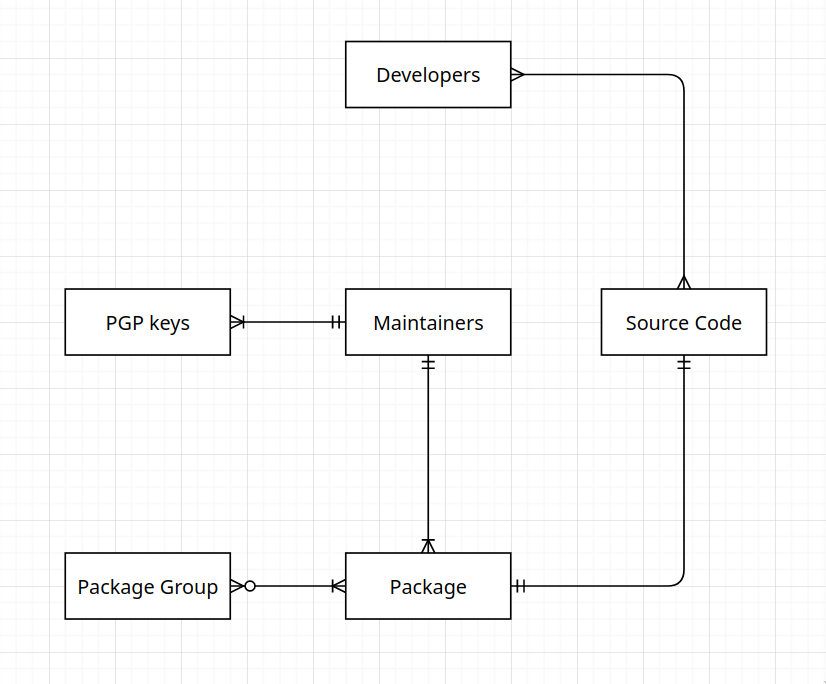
\includegraphics[scale=0.42]{repo-packages.png}}
    \caption{Концептуальная модель}
    \label{fig:image}
\end{figure}

\newpage

\section{Логическая модель}

Проектируемая база находится в 3НФ.

\begin{figure}[h]
    \center{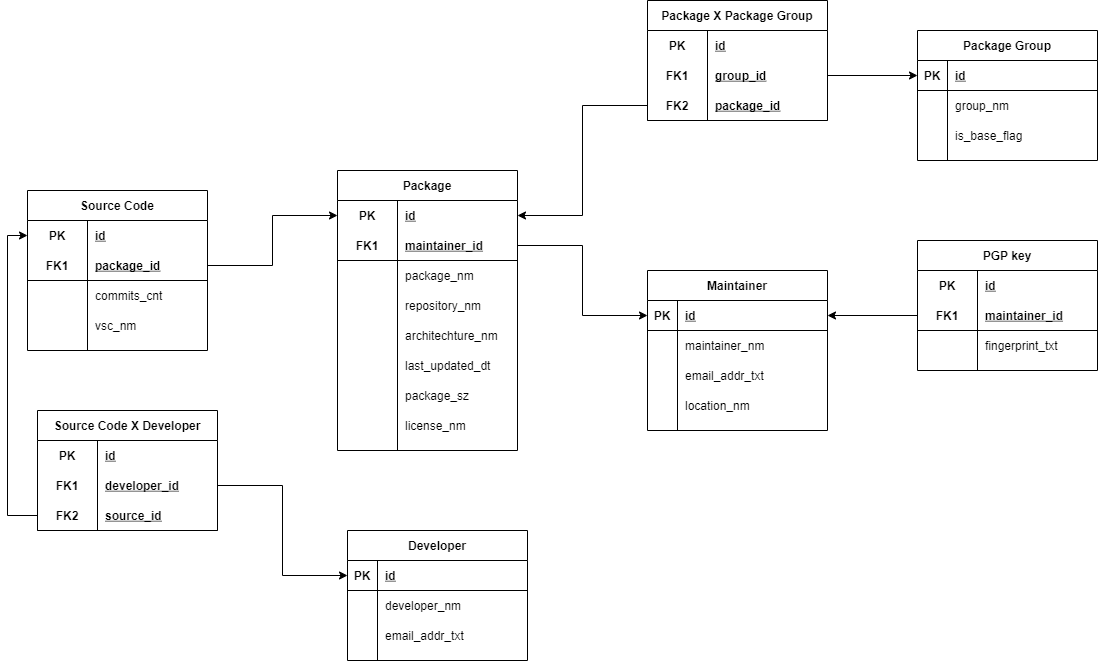
\includegraphics[scale=0.44]{logical-model.png}}
    \caption{Логическая модель (ER-диаграмма)}
    \label{fig:image}
\end{figure}

\newpage

\section{Физическая модель}


\begin{table}[h]
\centering
\resizebox{\textwidth}{!}{%
\begin{tabular}{|l|l|c|c|c|c|}
\hline
\multicolumn{6}{|c|}{\textbf{Maintainer}} \\ \hline
\multicolumn{1}{|c|}{\textbf{Название}} & \multicolumn{1}{c|}{\textbf{Описание}} & \textbf{Тип данных} & \textbf{Ограничение} & \textbf{PK} & \textbf{FK} \\ \hline
id & Уникальный ключ & SERIAL & NOT NULL & + &  \\ \hline
maintainer\_nm & Имя и фамилия мэйнтейнера & VARCHAR(128) & NOT NULL &  &  \\ \hline
email\_addr\_txt & Адрес электронной почты & TEXT &  &  &  \\ \hline
location\_nm & Страна проживания & VARCHAR(64) & NOT NULL &  &  \\ \hline
\end{tabular}%
}
\caption{Сущность Maintainer}
\label{my-label}
\end{table}


\begin{table}[h]
\centering
\resizebox{\textwidth}{!}{%
\begin{tabular}{|l|l|c|c|c|c|}
\hline
\multicolumn{6}{|c|}{\textbf{Package}} \\ \hline
\multicolumn{1}{|c|}{\textbf{Название}} & \multicolumn{1}{c|}{\textbf{Описание}} & \textbf{Тип данных} & \textbf{Ограничение} & \textbf{PK} & \textbf{FK} \\ \hline
id & Уникальный ключ & SERIAL & NOT NULL & + &  \\ \hline
maintainer\_id & Внешний ключ сущности мэйнтенер & INT & NOT NULL &  & + \\ \hline
package\_nm & Название пакета & VARCHAR(128) & NOT NULL &  &  \\ \hline
repository\_nm & Название репозитория, содержащего пакет & VARCHAR(16) & NOT NULL &  &  \\ \hline
architechture\_nm & Под какую архитектуру & VARCHAR(16) & NOT NULL &  &  \\ \hline
last\_updated\_dt & Дата последнего обновления & DATE & NOT NULL &  &  \\ \hline
package\_sz & Размер пакета в МБ & REAL & NOT NULL &  &  \\ \hline
license\_nm & Лицензия распространения & VARCHAR(16) & NOT NULL &  &  \\ \hline
\end{tabular}%
}
\caption{Сущность Package}
\label{my-label}
\end{table}


\begin{table}[h]
\centering
\resizebox{\textwidth}{!}{%
\begin{tabular}{|l|l|c|c|c|c|}
\hline
\multicolumn{6}{|c|}{\textbf{PGP key}} \\ \hline
\multicolumn{1}{|c|}{\textbf{Название}} & \multicolumn{1}{c|}{\textbf{Описание}} & \textbf{Тип данных} & \textbf{Ограничение} & \textbf{PK} & \textbf{FK} \\ \hline
id & Уникальный ключ & SERIAL & NOT NULL & + &  \\ \hline
maintainer\_id & Внешний ключ сущности мэйнтейнер & INT & NOT NULL &  & + \\ \hline
fingerprint\_txt & Хеш публичного ключа & VARCHAR(64) & NOT NULL, UNIQUE &  &  \\ \hline
\end{tabular}%
}
\caption{Сущность PGP key}
\label{my-label}
\end{table}


\begin{table}[h!]
\centering
\resizebox{\textwidth}{!}{%
\begin{tabular}{|l|l|c|c|c|c|}
\hline
\multicolumn{6}{|c|}{\textbf{Source Code}} \\ \hline
\multicolumn{1}{|c|}{\textbf{Название}} & \multicolumn{1}{c|}{\textbf{Описание}} & \textbf{Тип данных} & \textbf{Ограничение} & \textbf{PK} & \textbf{FK} \\ \hline
id & Уникальный ключ & SERIAL & NOT NULL & + &  \\ \hline
package\_id & Внешний ключ сущности пакет & INT & NOT NULL &  & + \\ \hline
commits\_cnt & Количество выполненых коммитов & INT & NOT NULL, DEFAULT 0, \textgreater{}= 0 &  &  \\ \hline
vcs\_nm & Название системы контроля верский & VARCHAR(16) & NOT NULL &  &  \\ \hline
\end{tabular}%
}
\caption{Сущность Source Code}
\label{my-label}
\end{table}


\begin{table}[h!]
\centering
\resizebox{\textwidth}{!}{%
\begin{tabular}{|l|l|c|c|c|c|}
\hline
\multicolumn{6}{|c|}{\textbf{Developer}} \\ \hline
\multicolumn{1}{|c|}{\textbf{Название}} & \multicolumn{1}{c|}{\textbf{Описание}} & \textbf{Тип данных} & \textbf{Ограничение} & \textbf{PK} & \textbf{FK} \\ \hline
id & Уникальный ключ & SERIAL & NOT NULL & + &  \\ \hline
developer\_nm & Имя разработчика & VARCHAR(128) & NOT NULL &  & \\ \hline
email\_addr\_txt & Адрес электронной почты & TEXT &  &  &  \\ \hline
\end{tabular}%
}
\caption{Сущность Developer}
\label{my-label}
\end{table}


\begin{table}[h!]
\centering
\resizebox{\textwidth}{!}{%
\begin{tabular}{|l|l|c|c|c|c|}
\hline
\multicolumn{6}{|c|}{\textbf{Source Code X Developer}} \\ \hline
\multicolumn{1}{|c|}{\textbf{Название}} & \multicolumn{1}{c|}{\textbf{Описание}} & \textbf{Тип данных} & \textbf{Ограничение} & \textbf{PK} & \textbf{FK} \\ \hline
id & Уникальный ключ & SERIAL & NOT NULL & + &  \\ \hline
developer\_id & Внешний ключ сущности разрабочика & INT &  &  & + \\ \hline
source\_id & Внешний ключ сущности исходного кода & INT &  &  & + \\ \hline
\end{tabular}%
}
\caption{Сущность Source Code X Developer}
\label{my-label}
\end{table}


\begin{table}[h!]
\centering
\resizebox{\textwidth}{!}{%
\begin{tabular}{|l|l|c|c|c|c|}
\hline
\multicolumn{6}{|c|}{\textbf{Package Group}} \\ \hline
\multicolumn{1}{|c|}{\textbf{Название}} & \multicolumn{1}{c|}{\textbf{Описание}} & \textbf{Тип данных} & \textbf{Ограничение} & \textbf{PK} & \textbf{FK} \\ \hline
id & Уникальный ключ & SERIAL & NOT NULL & + &  \\ \hline
group\_nm & Название группы & VARCHAR(16) & NOT NULL &  &  \\ \hline
is\_default\_flag & Входит ли в базовую установку & BOOLEAN & NOT NULL, DEFAULT FALSE  &  &  \\ \hline
\end{tabular}%
}
\caption{Сущность Package group}
\label{my-label}
\end{table}


\begin{table}[h!]
\centering
\resizebox{\textwidth}{!}{%
\begin{tabular}{|l|l|c|c|c|c|}
\hline
\multicolumn{6}{|c|}{\textbf{Package X Package Group}} \\ \hline
\multicolumn{1}{|c|}{\textbf{Название}} & \multicolumn{1}{c|}{\textbf{Описание}} & \textbf{Тип данных} & \textbf{Ограничение} & \textbf{PK} & \textbf{FK} \\ \hline
id & Уникальный ключ & SERIAL & NOT NULL & + &  \\ \hline
package\_id & Внешний ключ пакета & INT & NOT NULL & &  \\ \hline
group\_id & Внешний ключ группы пакетов & INT & NOT NULL & &  \\ \hline
\end{tabular}%
}
\caption{Сущность Package X Package Group}
\label{my-label}
\end{table}



\hfill \break
\hfill \break
\hfill \break
\hfill \break
\hfill \break

\end{document}
